\documentclass[tikz,border=8pt]{standalone}
\usepackage{amsmath}\usepackage{pgfplots}\pgfplotsset{compat=1.18}\usetikzlibrary{arrows.meta}
\definecolor{ink}{HTML}{334155}\definecolor{blue}{HTML}{6366F1}\definecolor{green}{HTML}{059669}\definecolor{orange}{HTML}{EA580C}
\begin{document}
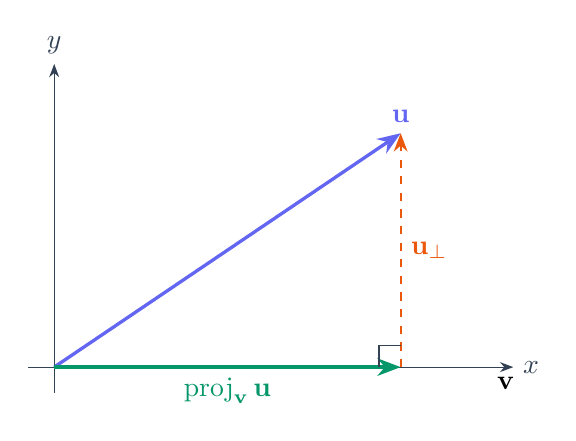
\begin{tikzpicture}[>=Stealth,scale=1.1]
\draw[->,ink] (-.3,0)--(5.3,0) node[right]{$x$};\draw[->,ink](0,-.3)--(0,3.5)node[above]{$y$};
\draw[very thick,->,blue](0,0)--(4,2.7)node[above]{$\mathbf u$};
\draw[very thick,->,green](0,0)--(4,0)node[below,midway]{$\operatorname{proj}_{\mathbf v}\mathbf u$};
\draw[thick,dashed,orange,->](4,0)--(4,2.7)node[right,midway]{$\mathbf u_\perp$};
\draw[ink](3.75,0)--(3.75,.25)--(4,.25);\node[below right]at(5,0){$\mathbf v$};
\end{tikzpicture}
\end{document}
